Einstein’s 1905 formulation of Special Relativity omitted the luminiferous æther as a mechanical necessity for light propagation. This has often been misinterpreted as a categorical rejection of any æther concept. However, Einstein’s statement was more nuanced:
\begin{quote}
    ``The introduction of a 'light-bearer' æther proves to be superfluous.''
\end{quote}

This does not deny the possibility that space possesses structure or physical attributes. Instead, it marks a shift from a mechanical to a field-theoretic perspective, not an ontological negation of any spacetime substrate. As explored in Section~\ref{sec:einstein_return}, Einstein would later revisit and explicitly refine the æther concept in the context of General Relativity.

This perspective—where space retains structure but not particulate substance—prefigures the modern VAM approach, in which the æther is formalized as a quantized, topological superfluid (see Sec.~\ref{sec:connection_to_VAM}, and~\cite{VAM-8}).

\section{The Return of the Æther Concept (1920)}
\label{sec:einstein_return}

Einstein’s 1920 Leiden lecture marks a critical clarification:
\begin{quote}
    ``According to the general theory of relativity, space is endowed with physical qualities; in this sense, therefore, there exists an æther. According to the general theory of relativity, space without æther is unthinkable.''~\cite{einstein1920aether}
\end{quote}

In this revised conception, the æther is not a mechanical substance but a geometric and energetic substrate. It carries properties such as curvature, stress-energy, and gravitational potential, and is inseparable from the fabric of spacetime. This evolution in Einstein’s thought forms the philosophical foundation for VAM, which regards the æther as a structured, dynamically active fluid rather than an inert void~\cite{VAM-8}.

In what follows, we examine Einstein’s later writings in this light and develop a fluid-dynamical continuation of his geometric intuition—now realized as a quantized, topologically rich superfluid with explicit links to particle physics and cosmology.
This connects with a broader tradition of analogue gravity models using superfluid or condensed-matter systems to model spacetime phenomena~\cite{barcelo2005}.


\section{Æther as Carrier of Field Quality}

Einstein explicitly redefined the æther in his later writings as a non-material but physically active entity. He emphasized that this æther:
\begin{itemize}
    \item Not composed of discrete particles,
    \item Not endowed with a state of absolute rest,
    \item Yet responsible for observable effects such as gravitation, field propagation, and the progression of time.
\end{itemize}

This interpretation departs from the 19th-century particulate æther, aligning instead with a modern view of the vacuum as a continuous, structured
background. The VAM framework adopts this perspective, modeling space as a (nearly) incompressible, inviscid superfluid in which all forces, fields, and even quantum phenomena emerge from topologically conserved vorticity and structured swirl~\cite{VAM-8, VAM-1, VAM-2}. VAM extends insights from analog condensed matter systems~\cite{volovik2003universe}, where emergent geometry and low-energy excitations mimic gravitational and cosmological phenomena.


\vspace{0.7em}
\noindent\textbf{Recent Results:}
Mathematically, these ideas are realized in VAM by:
\begin{itemize}
    \item Explicit definitions of absolute time (\(\boldsymbol{\mathcal{N}}\)), proper time (\(\boldsymbol{\tau}\)), and internal phase clocks (\(\boldsymbol{S}^{\boldsymbol{\circlearrowleft}}_\text{(t)}\)), as rigorously formulated in~\cite{VAM-8, VAM-1}.
    \item Derivation of gravitational and inertial effects from swirl-induced pressure gradients, replacing geometric curvature in General Relativity (see~\cite{VAM-2, VAM-3, VAM-8}).
    \item A vortex mass equation relating particle rest masses to vortex topology~\cite{widnall1973vortexrings}, and a complete knot taxonomy for all Standard Model particles~\cite{VAM-8, VAM-11}.This continues the foundational work on knot theory in fluid mechanics, where helicity and topological conservation are central to vortex structure~\cite{knot_theroy_in_fluid}.

    \item Direct empirical benchmarking of VAM predictions for time dilation, redshift, frame-dragging, and cosmological phenomena (see~\cite{VAM-3, VAM-8}).
    \item Formulation of a unified topological Lagrangian encompassing all known interactions (see~\cite{VAM-14}).
\end{itemize}

In this view, the metric tensor and curvature of GR become emergent, large-scale approximations of the underlying vortex field dynamics—a hypothesis now rendered testable and falsifiable through precise mathematical and observational correspondence (see ~\ref{sec:lorentz_recovery}, and~\cite{VAM-8, VAM-3}), similar in spirit to emergent gravity approaches where spacetime arises from thermodynamic or information-theoretic principles~\cite{Verlinde2011}. This parallels current efforts to probe the microstructure of spacetime and challenge the foundational assumptions of geometry-driven field theories~\cite{hossenfelder2018lost}.

This historical development of mass ontology—from atomic substance to structured vorticity—is depicted in Figure~\ref{fig:OntologyOfMass}.


\begin{figure}[htbp]
      \centering
    \scriptsize
    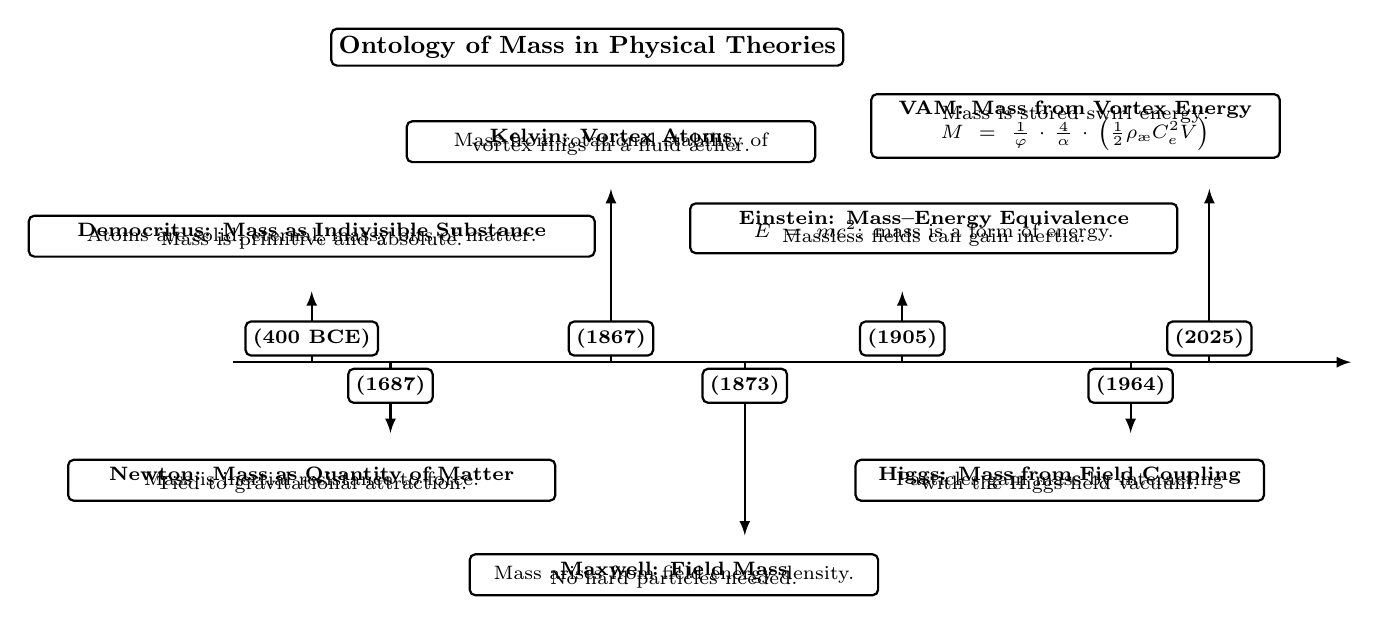
\begin{tikzpicture}[node distance=3.5cm, every node/.style={font=\scriptsize}, >=latex]
    \scriptsize

    % Timeline base
    \draw[->, thick] (-1,0) -- (13.2,0);

    % Arrows above timeline (short, as requested)
    \draw[->, thick] (0,0) -- (0,0.9);       % Pre-Socratics
    \draw[->, thick] (3.8,0) -- (3.8,2.2);   % Augustine
    \draw[->, thick] (7.5,0) -- (7.5,0.9);   % Einstein
    \draw[->, thick] (11.4,0) -- (11.4,2.2); % VAM

    % Arrows below timeline (short, as requested)
    \draw[->, thick] (1.0,0) -- (1.0,-0.9);     % Plato/Aristotle
    \draw[->, thick] (5.5,0) -- (5.5,-2.2);     % Newton
    \draw[->, thick] (10.4,0) -- (10.4,-0.9);     % Leibniz/Mach

        %--- Root title cards (above timeline) ---
    \node[draw, thick, rounded corners=2pt, fill=white, align=center, font=\bfseries ] at (0, .3)   {(400 BCE)};
    \node[draw, thick, rounded corners=2pt, fill=white, align=center, font=\bfseries ] at (3.8, .3) {(1867)};
    \node[draw, thick, rounded corners=2pt, fill=white, align=center, font=\bfseries ] at (7.5, .3) {(1905)};
    \node[draw, thick, rounded corners=2pt, fill=white, align=center, font=\bfseries ] at (11.4, .3){(2025)};

    %--- Root title cards (below timeline) ---
    \node[draw, thick, rounded corners=2pt, fill=white, align=center, font=\bfseries ] at (1.0,- .3) {(1687)};
    \node[draw, thick, rounded corners=2pt, fill=white, align=center, font=\bfseries ] at (5.5,- .3) {(1873)};
    \node[draw, thick, rounded corners=2pt, fill=white, align=center, font=\bfseries ] at (10.4,- .3) {(1964)};

    % Label
    \node[draw, thick, fill=white, rounded corners=2pt, font=\small] at (3.5,4.0) {\textbf{Ontology of Mass in Physical Theories}};

    % Democritus (left)
    \node[draw, rounded corners=2pt, thick, align=center, fill=white, text width=7cm] at (0,1.6) {
    \textbf{Democritus: Mass as Indivisible Substance}  \\[-0.8em]
    Atoms are solid, eternal, massy bits of matter.  \\[-0.8em]
    Mass is primitive and absolute.
    };

    % Newton (below)
    \node[draw, rounded corners=2pt, thick, align=center, fill=white, text width=6cm] at (0,-1.5) {
    \textbf{Newton: Mass as Quantity of Matter}  \\[-0.8em]
    Mass is inertial resistance to force.  \\[-0.8em]
    Tied to gravitational attraction.
    };


    % Kelvin (top)
    \node[draw, rounded corners=2pt, thick, align=center, fill=white, text width=5cm] at (3.8,2.8) {
    \textbf{Kelvin: Vortex Atoms}  \\[-0.8em]
    Mass from rotational stability of  \\[-0.8em]
    vortex rings in a fluid æther.
    };


    % Maxwell (bottom)
    \node[draw, rounded corners=2pt, thick, align=center, fill=white, text width=5cm] at (4.6,-2.7) {
    \textbf{Maxwell: Field Mass}  \\[-0.8em]
    Mass arises from field energy density.  \\[-0.8em]
    No hard particles needed.
    };

    % Einstein (top)
    \node[draw, rounded corners=2pt, thick, align=center, fill=white, text width=6cm] at (7.9,1.7) {
    \textbf{Einstein: Mass–Energy Equivalence}  \\[-0.4em]
    \( E = mc^2 \): mass is a form of energy.  \\[-0.8em]
    Massless fields can gain inertia.
    };


    % Higgs (bottom)
    \node[draw, rounded corners=2pt, thick, align=center, fill=white, text width=5cm] at (9.5,-1.5) {
    \textbf{Higgs: Mass from Field Coupling}  \\[-0.8em]
    Particles gain mass by interacting  \\[-0.8em]
    with the Higgs field vacuum.
    };


    % VAM (top right)
    \node[draw, rounded corners=2pt, thick, align=center, fill=white, text width=5cm] at (9.7,3.0) {
    \textbf{VAM: Mass from Vortex Energy}  \\[-0.8em]
    Mass is stored swirl energy:  \\[-0.4em]
    \( M = \frac{1}{\varphi} \cdot \frac{4}{\alpha} \cdot \left( \frac{1}{2} \rho_\text{\ae} C_e^2 V \right) \)
    };

    \end{tikzpicture}
    \caption{\textbf{Evolution of the concept of mass across physics:} from atomistic substance (Democritus), through Newtonian inertia and field-theoretic mass (Maxwell, Higgs), to VAM’s fluid-topological model. In VAM, mass is emergent swirl energy stored in knotted vortex configurations within a quantized æther. Each stage reflects deeper abstraction—from particles to energy to geometry to topology.}\label{fig:OntologyOfMass}
\end{figure}

\section{Emergent Lorentz Symmetry from Swirl Fields}
\label{sec:lorentz_recovery}

While VAM posits an absolute æther frame \(\boldsymbol{\mathcal{N}}\), it nonetheless recovers Lorentz symmetry as an emergent approximation for observers embedded within stable vortex structures. This effective symmetry arises from local swirl-induced time dilation, governed by the relation:
\begin{equation}
    d\tau = dt \sqrt{1 - \frac{|\vec{\omega}|^2}{c^2}},
\end{equation}
which mimics the classical Lorentz contraction formula \(dt' = dt \sqrt{1 - v^2/c^2}\) when angular swirl velocity \(|\vec{\omega}|\) is interpreted as a local velocity surrogate.

\begin{figure}[htbp]
      \centering
    \scriptsize
        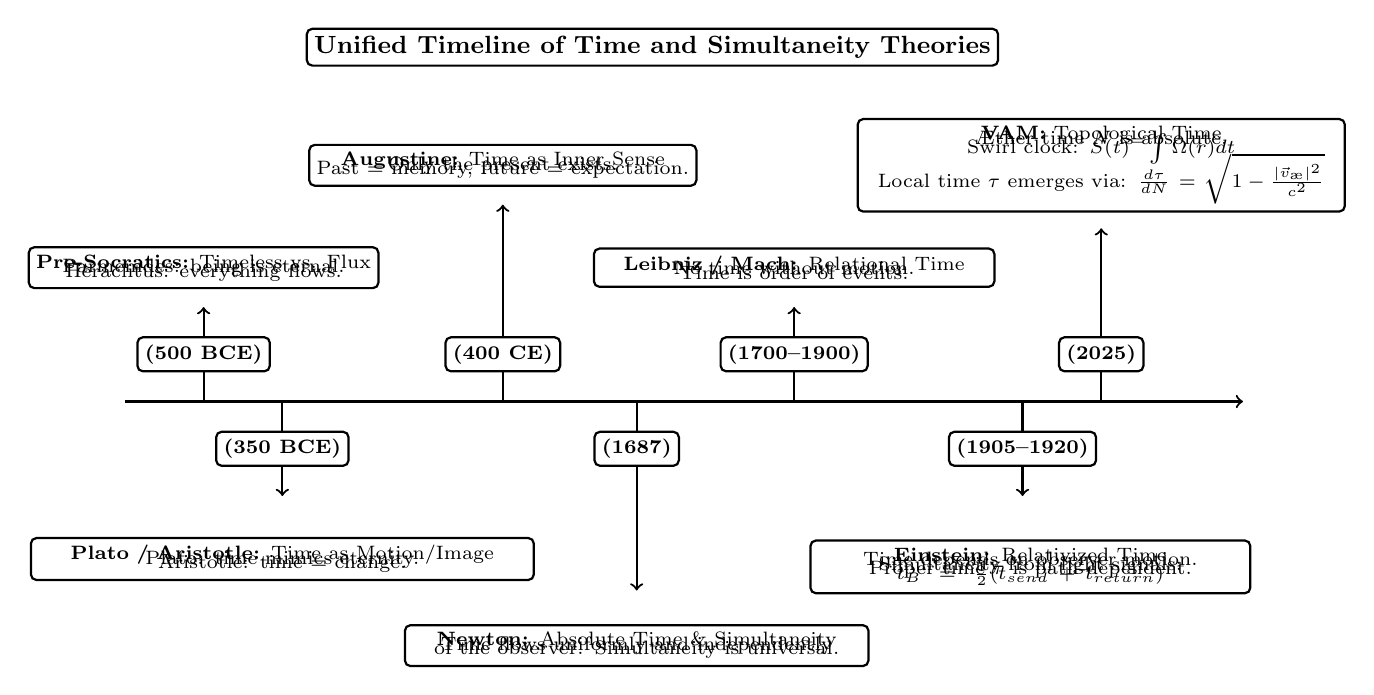
\begin{tikzpicture}
        \scriptsize
        % Timeline base
        \draw[->, thick] (-1,0) -- (13.2,0);

        % Arrows above timeline (short, as requested)
        \draw[->, thick] (0,0) -- (0,1.2);       % Pre-Socratics
        \draw[->, thick] (3.8,0) -- (3.8,2.5);   % Augustine
        \draw[->, thick] (7.5,0) -- (7.5,1.2);   % Einstein
        \draw[->, thick] (11.4,0) -- (11.4,2.2); % VAM

        % Arrows below timeline (short, as requested)
        \draw[->, thick] (1.0,0) -- (1.0,-1.2);     % Plato/Aristotle
        \draw[->, thick] (5.5,0) -- (5.5,-2.4);     % Newton
        \draw[->, thick] (10.4,0) -- (10.4,-1.2);     % Leibniz/Mach

            %--- Root title cards (above timeline) ---
        \node[draw, thick, rounded corners=2pt, fill=white, align=center, font=\bfseries ] at (0, .6)   {(500 BCE)};
        \node[draw, thick, rounded corners=2pt, fill=white, align=center, font=\bfseries ] at (3.8, .6) {(400 CE)};
        \node[draw, thick, rounded corners=2pt, fill=white, align=center, font=\bfseries ] at (7.5, .6) {(1700--1900)};
        \node[draw, thick, rounded corners=2pt, fill=white, align=center, font=\bfseries ] at (11.4, .6){(2025)};

        %--- Root title cards (below timeline) ---
        \node[draw, thick, rounded corners=2pt, fill=white, align=center, font=\bfseries ] at (1.0,- .6) {(350 BCE)};
        \node[draw, thick, rounded corners=2pt, fill=white, align=center, font=\bfseries ] at (5.5,- .6) {(1687)};
        \node[draw, thick, rounded corners=2pt, fill=white, align=center, font=\bfseries ] at (10.4,- .6) {(1905--1920)};

            % Timeline label
        \node[draw, thick, fill=white, rounded corners=2pt, font=\small] at (5.7,4.5) {\textbf{Unified Timeline of Time and Simultaneity Theories}};

        % --- Pre-Socratics ---
        \node[draw, rounded corners=2pt, thick, align=center, fill=white] at (0,1.7) {
        \textbf{Pre-Socratics:} Timeless vs. Flux \\[-0.8em]
        Parmenides: being is eternal. \\[-0.8em]
        Heraclitus: everything flows.
        };

        % --- Augustine ---
        \node[draw, rounded corners=2pt, thick, align=center, fill=white] at (3.8,3.0) {
        \textbf{Augustine:} Time as Inner Sense \\[-0.8em]
        Only the present exists. \\[-0.8em]
        Past = memory, future = expectation.
        };

        % --- Leibniz / Mach ---
        \node[draw, rounded corners=2pt, thick, align=center, fill=white, text width=4.9cm] at (7.5,1.7) {
        \textbf{Leibniz / Mach:} Relational Time \\[-0.8em]
        No time without motion. \\[-0.8em]
        Time is order of events.
        };
        % --- VAM (modern) ---
        \node[draw, rounded corners=2pt, thick, align=center, fill=white, text width=6.0cm] at (11.4,3.0) {
        \textbf{VAM:} Topological Time \\[-0.8em]
        Æther time $N$ is absolute. \\[-0.6em]
        Swirl clock: $S(t)^\circlearrowleft = \int \Omega(r) dt$ \\[-0.6em]
        Local time $\tau$ emerges via: $ \frac{d\tau}{dN} = \sqrt{1 - \frac{|\vec{v}_\text{\ae}|^2}{c^2}}$

        };


        % --- Plato / Aristotle ---
        \node[draw, rounded corners=2pt, thick, align=center, fill=white, text width=6.2cm] at (1.0,-2) {
        \textbf{Plato / Aristotle:} Time as Motion/Image \\[-0.8em]
        Plato: time mimics eternity. \\[-0.8em]
        Aristotle: time = change.
        };



        % --- Einstein ---
        \node[draw, rounded corners=2pt, thick, align=center, fill=white, text width=5.4cm] at (10.5,-2.1) {
        \textbf{Einstein:} Relativized Time \\[-0.8em]
        Time depends on observer motion. \\[-0.8em]
        Simultaneity from light signals: \\[-0.8em]
        Proper time $\tau$ is path-dependent.\\[-0.8em]
        $t_B = \frac{1}{2}(t_{\text{send}} + t_{\text{return}})$
        };

        % --- Newton ---
        \node[draw, rounded corners=2pt, thick, align=center, fill=white, text width=5.7cm] at (5.5,-3.1) {
        \textbf{Newton:} Absolute Time \& Simultaneity \\[-0.8em]
        Time flows uniformly and independently \\[-0.8em]
        of the observer. Simultaneity is universal.
        };
         \end{tikzpicture}
        \caption{Fused history of time and simultaneity: from early philosophical views and Newton’s absolutes to Einstein’s relativistic structure and VAM’s layered, swirl-based temporality.}\label{fig:history-time-simultaneity}
\end{figure}


Figure~\ref{fig:history-time-simultaneity} traces the evolving notions of simultaneity and time—from Newton’s absolutes to Einstein’s relativity and the layered temporality of VAM.
Swirl clocks \(S^{\circlearrowleft}_\text{(t)}\) advance slower in regions of high vorticity, reproducing relativistic effects such as time dilation, redshift, and frame dragging. However, unlike in special relativity, these effects are not fundamental symmetries of spacetime but fluid-mechanical consequences of structured vortex motion.

This reinterpretation demotes Lorentz invariance from an a priori principle to a derivative, scale-dependent symmetry—a conclusion supported by multiple derivations across the VAM corpus~\cite{VAM-1, VAM-2, VAM-15}.

\vspace{0.8em}

\noindent\textbf{Ætheric Temporal Sequence:}
\begin{center}
\(\boldsymbol{\mathcal{N}} \to \boldsymbol{\nu_0} \to \boldsymbol{\tau} \to \boldsymbol{S}^{\boldsymbol{\circlearrowleft}}_\text{(t)} \to \boldsymbol{T_v} \to \mathbb{\boldsymbol{K}}\)
\end{center}